% vim: spelllang=fr

\documentclass[../main.tex]{subfiles}
\graphicspath{{\subfix{../Figures/Chap2/}}}
\begin{document}

\begin{itshape}
Ce deuxième chapitre porte de l'approche directe consistant en l'application d'un algorithme de détection et de suivi des cyclones tropicaux dans les modèles
comme façon de caractériser l'activité cyclonique simulée, ainsi que la façon dont les modèles représentent ces phénomènes. Un cas d'étude est présenté via
l'application du schéma de détection du CNRM à la réanalyse ERA5.
\end{itshape}

\minitoc\newpage
%--------------------------------------
\section{Évaluation du traqueur CNRM sur ERA5 par rapport à IBTrACS}\label{sec:eval_tracker_ERA5}

\subsection{Introduction}

Les algorithmes de détection et de suivi des HTV dans les modèles consistent à identifier les points de grille qui satisfont des critères thermiques ou
dynamiques associés à un cyclone tropical. Le \cref{chap:chapitre_1}, en particulier la \cref{sec:intro_tracking}, met en évidence la sensibilité de l'activité
cyclonique mesurée au choix de la méthode de détection et montre que ce choix peut aboutir à des conclusions différentes quant au signe du changement dans des
expériences à climat plus chaud. Les premiers schémas de détection étaient basés uniquement sur la MSLP et la vitesse des vents
\parencite{bengtsson_simulation_1982,broccoli_can_1990}, tandis que \cite{haarsma_tropical_1993,bengtsson_hurricanetype_1995} ajoutèrent à cela des critères sur
la vorticité ainsi qu'un diagnostique sur la présence d'un cœur chaud, dans l'optique de discriminer les perturbations tropicales de leurs homologues
extra-tropicales. \cite{wu_gcm_1992} utilisèrent des critères supplémentaires conçus pour discriminer les perturbations tropicales sèches via un seuil
d'humidité relative, les perturbations équatoriales d'est en interdisant le vent d'est à \hPa{950} au point situé à \ang{4.5} au nord et au sud du cyclone,
ainsi que les perturbations barocliniques en bornant la vitesse du vent d'ouest à \hPa{200} au dessus du centre du cyclone à \ms{5}. Dans
\cite{bengtsson_hurricanetype_1995}, la méthodologie de détection introduit des tests de structure verticale du système, aussi bien sur le profil de vent que de
température. En effet, après avoir identifié un centre cyclonique à travers la vorticité, pression minimum locale et vitesse du vent maximale dans une boîte
autour du système, il s'agit alors de s'assurer de la présence d'une anomalie de température sur l'ensemble de la troposphère, par rapport à la moyenne prise
dans cette boîte, puis de s'assurer également que l'anomalie à la tropopause est supérieure que celle à la couche limite. Un test similaire est réalisé sur le
profil vertical de vent, en imposant que le vent moyen à \hPa{850} supérieur à la moyenne du niveau à \hPa{300}, toujours dans la boîte. Beaucoup d'algorithmes
de détection reprennent cette méthodologie, avec quelques variantes et spécificités. Une grande quantité de méthodologies et de seuils de détection sont décrits
dans \cite{walsh_objectively_2007} ainsi que dans \cite[][Annexe B]{ullrich_tempestextremes_2017}.

Le schéma de détection TRACK \parencite{hodges_how_2017}, très couramment utilisé, a par exemple la particularité de systématiquement interpoler les champs du
modèle à une basse résolution (T63, soit \km{210}), avant d'appliquer un schéma de détection basé exclusivement sur la vorticité. Cela permettrait de
s'affranchir de la sensibilité de la méthode de détection à la résolution du modèle. Cet algorithme a cependant tendance à détecter une quantité parfois
anormalement élevée de systèmes (voir \cref{fig:NTC_HighResMIP_TRACK} par rapport à la \cref{fig:NTC_HighResMIP}), et est alors particulièrement sujet à la
détection de faux-positifs \parencite{bourdin_intercomparison_2022}. La problématique que TRACK vise à solutionner est néanmoins bien réelle. La résolution du
modèle impacte la représentation des TC dans les modèles ce qui implique que les seuils de détection nécessitent d'être ajustés à la résolution du modèle, et
sont en pratique souvent ajustés empiriquement de manière à reproduire la climatologie observée \parencite{walsh_objectively_2007,tory_development_2013}. Pour
répondre à cette problématique, \cite{camargo_improving_2002} ont proposé une méthoque de détection de HTV dont les seuils pour chacunes des variables sont
déterminées à partir de la climatologie du modèle. Spécifiquement, ces derniers s'expriment sous la forme $\alpha \sigma + \beta$, où $\alpha$ et $\beta$ sont
issues de la climatologie globale du modèle, et où $\sigma$ représente l'écart type de la variable à l'échelle de chaque bassin océanique. La méthode de
\cite{camargo_improving_2002} n'est cependant pas largement répandue, possiblement parce que d'une part, les valeurs $\alpha$ et $\beta$ pour chacune des
variables se déterminent par les densités de probabilités bivariées dont l'estimation est complexe et laborieuse, et d'autre part parce que cette approche
représente un paradigme très différent des traqueurs mentionnés précédemment. En effet, les traqueurs à seuils fixes visent à appliquer un schéma de
fonctionnement conceptuel d'un cyclone tropical au modèle, ce qui permet ensuite d'établir dans quelle mesure le modèle est capable de simuler ces systèmes, là
où la méthode de \cite{camargo_improving_2002} cherche au contraire à s'affranchir des biais intrinsèques au modèle.

Une autre façon d'évaluer les performances d'un algorithme de détection et de suivi de cyclones tropicaux est de l'appliquer à une simulation dont les
trajectoires de TC sont connues d'avance, en utilisant une réanalyse atmosphérique.

\subsection{Résumé de l'article}

La réanalyse ERA5 du Centre européen pour les prévisions météorologiques à moyen terme est la première réanalyse mondiale à atteindre une résolution horizontale
de \km{31} et offre donc une occasion unique d'étudier les cyclones tropicaux, et en particulier les champs 3D associés aux TC historiques. A cette fin, un
algorithme de détection et de suivi des TC spécialement calibré pour ce jeu de données est appliqué sur ERA5 ainsi qu'un algorithme d'appariement des
trajectoires conçu pour associer les trajectoires détectées avec celles issues de la base de données IBTrACS dans le but d'évaluer la capacité de la réanalyse à
représenter les cyclones tropicaux Après optimisation du schéma de suivi et l'application d'une technique de filtrage dynamique des systèmes de moyennes
latitudes, il est montré que la majorité des TC d'IBTrACS sont détectés dans ERA5 et que le nombre de fausses alarmes reste raisonnablement bas dans la plupart
des régions. En comparant les trajectoires détectées dans ERA5 avec leurs équivalents IBTrACS, on constate que l'intensité des TC est encore fortement
sous-estimée dans la réanalyse, mais que la distribution de la pression minimale au niveau de la mer est mieux représentée que la vitesse maximale du vent. Par
ailleurs, la comparaison entre les cycles de vie des deux jeux de données met en évidence des différences essentielles entre ERA5 et les best tracks, avec en
particulier un retard avec lequel les TC d'ERA5 atteignent leur pic d'intensité par rapport à IBTrACS, délai qui augmente de manière significative pour les
cyclones les plus forts. Enfin, les structures verticales des TC dans la réanalyse sont analysées et révèlent une intensification nette jusqu'à la catégorie 3
sur l'échelle de Saffir-Simpson, au delà de quoi les différences sont peu discernables.

La version publiée de \cite{dulac_assessing_2023} est présentée dans la \cref{sec:papier} ci-après, avec la permission de l'éditeur \textit{Springer Nature}.

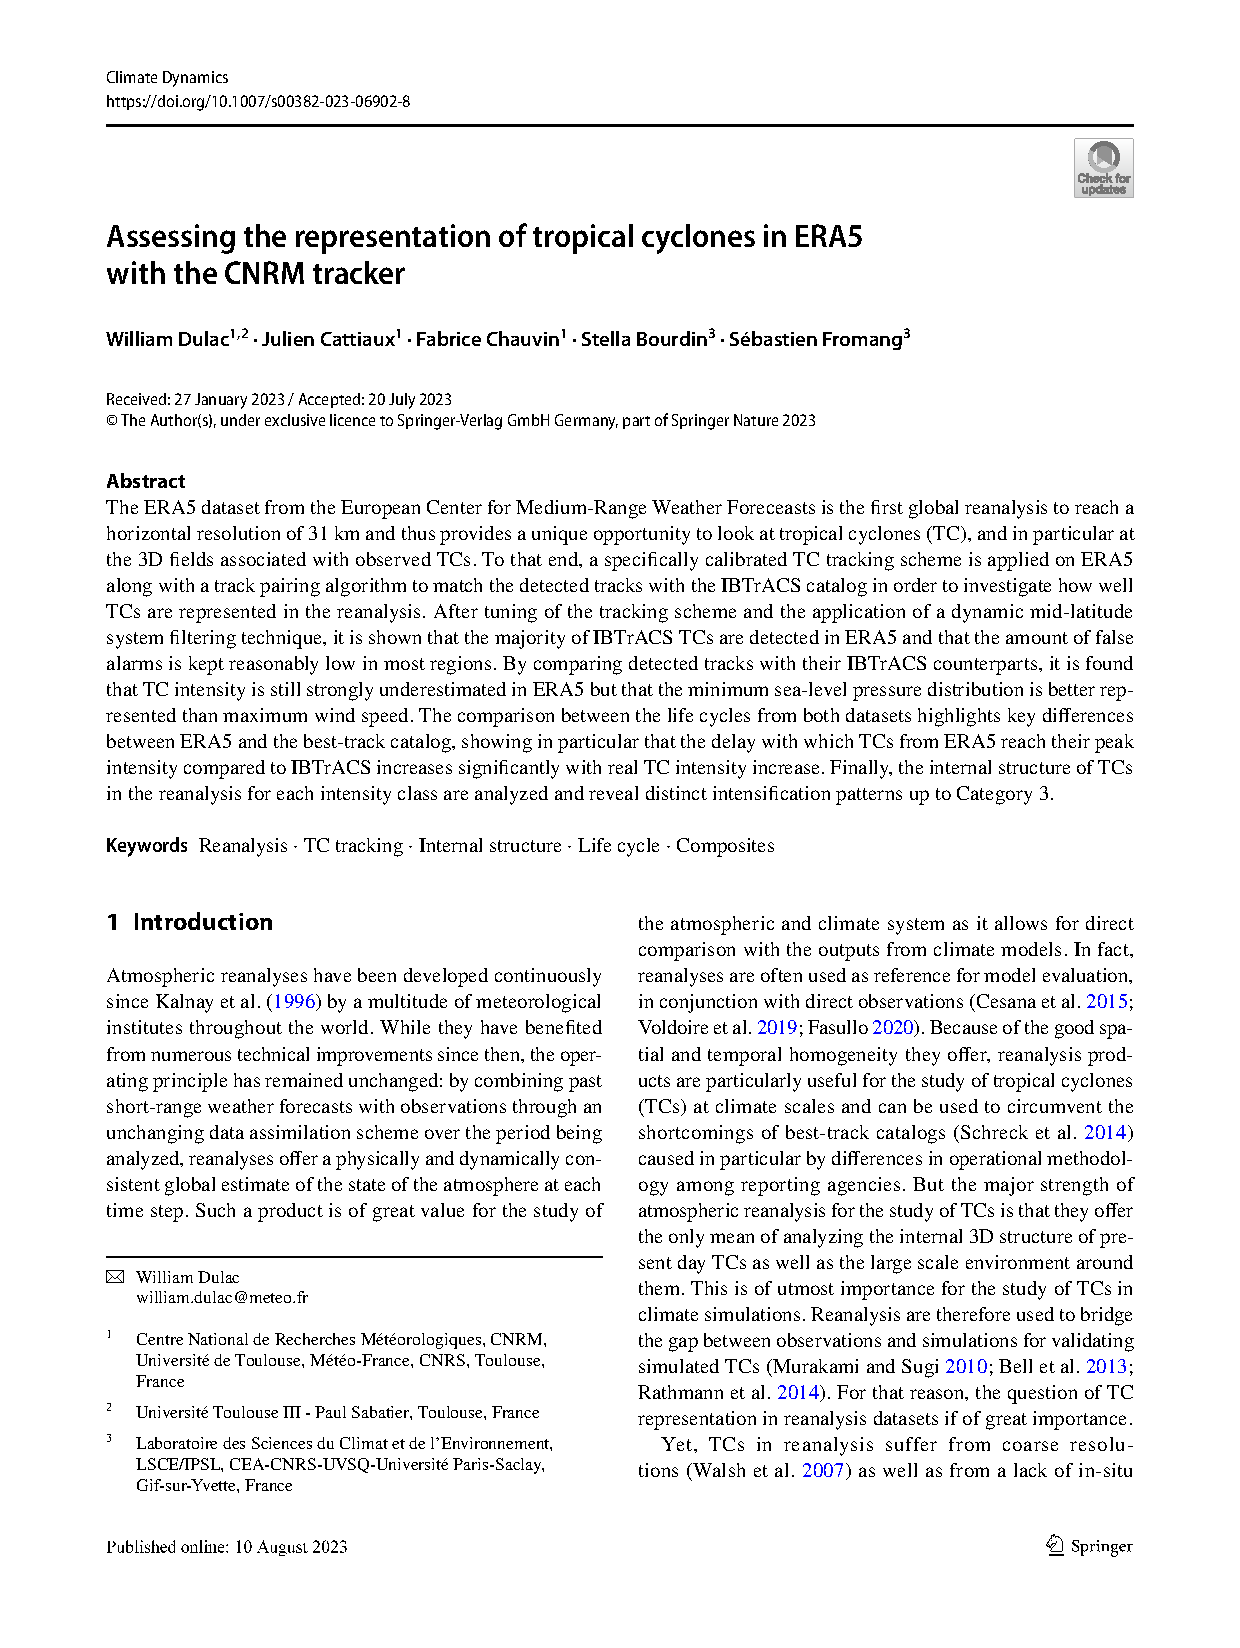
\includepdf[pages=-,pagecommand={\thispagestyle{plain}},offset=5mm 0mm,scale=1,addtotoc=
    {1,subsection,1,Article Climate Dynamics,sec:papier,
     1,subsubsection,2,Introduction,sec:papier_intro,
     2,subsubsection,2,Données et Méthodes,sec:papier_data_methods,
     4,subsubsection,2,Résultats,sec:papier_results,
     10,subsubsection,2,Discussion et conclusion,sec:papier:discussion,
     12,subsubsection,2,Annexe A: Optimisation du traqueur pour ERA5,sec:papier_appendix_A}]{\subfix{../include/dulac2023.pdf}}
%
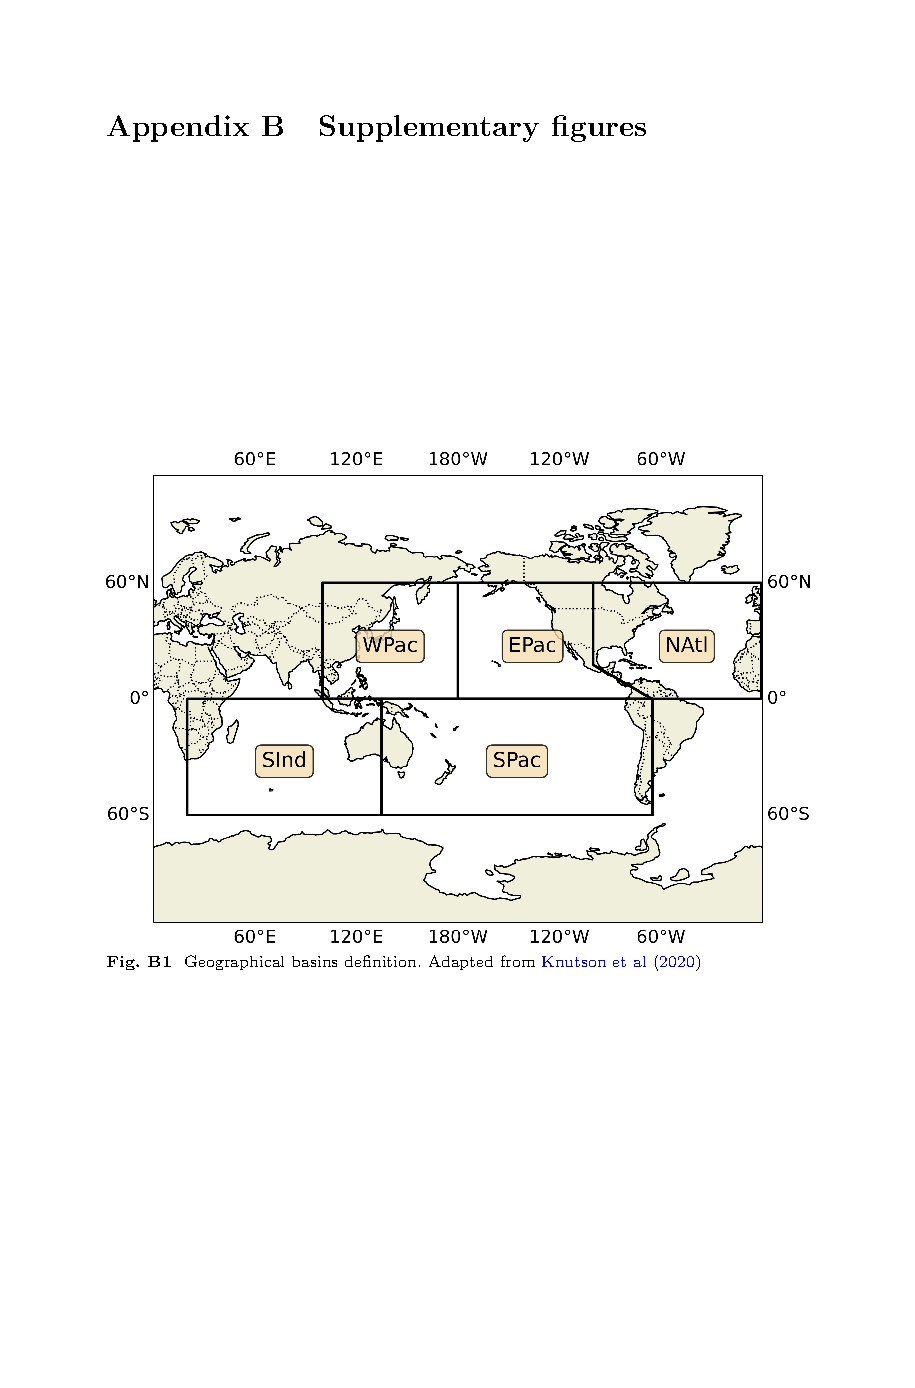
\includepdf[pages=-,pagecommand={\thispagestyle{plain}},offset=5mm 0mm,addtotoc=
{1,subsubsection,2,Annexe B: Figures supplémentaires,sec:papier_appendix_B}]{\subfix{../include/appendix_B_empty.pdf}}

\section{Compléments}

\subsection{Filtrage des systèmes de moyennes latitudes}\label{sec:filtrage_mid_latitudes}

\subsection{Métriques d'évaluation de la similarité des trajectoires}\label{sec:similarité}



%--------------------------------------
\section{Synthèse}

\end{document}
